\documentclass[twocolumn, a4paper]{article}

\usepackage{amsthm, amsmath, amssymb}
\usepackage{microtype}
\usepackage{graphicx}
\usepackage{booktabs} % for professional tables
\usepackage{hyperref}
\usepackage{multirow}
\usepackage{array}
\urlstyle{same}
\hypersetup{colorlinks=true, linkcolor=black, citecolor=black, urlcolor=blue}

\usepackage{subcaption}

\usepackage[top=2cm, bottom=2cm, left=1.5cm, right=1.5cm]{geometry}
\usepackage{titlesec}
    \titleformat{\title}{\large\bfseries}{}{}{}
    \titleformat{\section}{\normalfont\bfseries}{\thesection}{0.5em}{}
    \titleformat{\subsection}{\normalfont\it}{\thesubsection}{0.5em}{}
    \titleformat{\subsubsection}{\normalfont\normalsize\it}{\thesubsubsection}{0.5em}{}
    \titleformat{\paragraph}[runin]{\normalfont\bfseries}{\theparagraph}{0.5em}{}
    \titleformat{\subparagraph}[runin]{\normalfont\normalsize\it}{\thesubparagraph}{0.5em}{}
\usepackage[font=small,labelfont=bf,labelsep=space]{caption}

% \usepackage[ruled]{algorithm2e}
% \SetKwComment{Comment}{// }{ }

\usepackage{graphicx}
\graphicspath{{../assets}}

\usepackage{pgfplots}
\pgfplotsset{compat=1.18}

\pgfplotsset{
    report_style/.style={
    legend style={draw=none, font=\small},
    legend cell align=left,
    legend pos=north east,
    ylabel style={align=center, font=\bfseries\boldmath},
    xlabel style={align=center, font=\bfseries\boldmath},
    x tick label style={font=\bfseries\boldmath},
    y tick label style={font=\bfseries\boldmath},
    scaled ticks=false,
    every axis plot/.append style={thick},
    },
}

\usepackage{tikz}
\usetikzlibrary{shapes.geometric, arrows}
\usetikzlibrary{calc}
\usetikzlibrary{positioning}
\usetikzlibrary{fit}

\newtheorem{theorem}{Theorem}
\newtheorem{lemma}{Lemma}
\newtheorem{corollary}{Corollary}
\theoremstyle{definition}
\newtheorem{definition}{Definition}

\begin{document}

\title{\bf\Large Segmentation of 3D volume images for connectomics}
\author{Oleh Shkalikov\texorpdfstring{ (5102818)
\\[0.7em]{\small Supervisors: Jannik Irmai, David Stein}
\\{\small Chairholder: Prof. Dr. Bjoern Andres}}{}}
\date{CMS Research project, TU Dresden}

\twocolumn[
    \begin{@twocolumnfalse}
        \maketitle

        \vspace{7ex}
    \end{@twocolumnfalse}
]

\section{Introduction}
The aim of this research project is to develop approaches
for segmentation of 3D volume images for connectomics given
a labeled dataset. The importance of this problem comes from the
developing of methods (e.g. \cite{10.7554/eLife.25916}) of acquiring high resolution volume images
which makes hard to analyze all gathered data by hand because of their size.
Therefore automatic methods such as automatic labeling of data is needed.

In this work we will propose CNN based methods for solving this task and evaluate them
on the given dataset.

\section{Dataset description and analysis} \label{sec:data_analysis}

The labeled dataset which we use for out project is based on
the image volumes of the CA1 hippocampus region of the brain
acquired by a focused ion beam scanning electron microscope (FIB-SEM).
The raw data has a shape \( 2048 \times 1536 \times 1065 \)  and is available under
\url{https://www.epfl.ch/labs/cvlab/data/data-em/}. It was initially used in
\cite{lucchi2011supervoxel,lucchi2013learning} because this dataset also contains binary
labels for mitochondria which we don't use because we have been provided with wider
set of labels. The given connectomics volume image of the brain is
isotropic which allow us to rotate the volume/subvolumes without any side effects.

The actual labeling has been performed by An Dang Thanh (student of the MLCV lab)
only on slices of subvolumes where to
each pixel of slice \textbf{one} of the following labels has been assigned:
\begin{enumerate}
    \itemsep0em
    \item cell cytoplasm
    \item cell membrane
    \item mitochondrion
    \item mitochondrion membrane
    \item synapse
    \item vesicle
    \item undefined (in the case where annotator was uncertain about the correct label)
\end{enumerate}
In total 9 slices of the raw data volume has been labeled and split into train,
validation and test splits: 3 slices for each split, but every train slice has a shape
\( 600 \times 600 \) whereas every validation and test slice has a shape \( 425 \times 425 \).
The locations of slices in the raw volume are denoted in the table~\ref{tab:data_loc}.
\begin{table}[t]
    \centering
    \begin{tabular}{|c|c|c|c|}
        \hline
        \textbf{Split}                    & \textbf{X range}   & \textbf{Y range}   & \textbf{Z range}  \\
        \hline

        \multirow[vpos]{3}{*}{Train}      & \( [510, 1109] \)  & \( [200, 799] \)   & 200               \\
                                          & \( [510, 1109] \)  & 510                & \( [150, 749 ] \) \\
                                          & \( 595  \)         & \( [200, 799] \)   & \( [150, 749 ] \) \\
        \hline
        \multirow[vpos]{3}{*}{Validation} & \( [675, 1099] \)  & \( [1000, 1424] \) & 320               \\
                                          & \( [675, 1099] \)  & 1140               & \( [200, 624] \)  \\
                                          & \( 985  \)         & \( [1000, 1424] \) & \( [200, 624] \)  \\
        \hline
        \multirow[vpos]{3}{*}{Test}       & \( [1325, 1749] \) & \( [1000, 1424] \) & 650               \\
                                          & \( [1325, 1749] \) & 1100               & \( [350, 774 ] \) \\
                                          & \( 1532  \)        & \( [1000, 1424] \) & \( [350, 774 ] \) \\
        \hline
    \end{tabular}
    \caption{Location of the labeled slices in the raw volume}
    \label{tab:data_loc}
\end{table}

The dataset has been labeled by a non bio-medical expert, therefore there is a chance of mistakes
in the labeling. Another limitation of the dataset is the fact that the same pixel can represent
different biological structures and therefor labels whereas in our dataset we have only one label for
every pixel. For example, vesicles and mitochondria are part of the cell cytoplasm or
synapses are labeled as regions where a neuron passes a signal to another neuron and belong
to cell membranes and cell cytoplasm.

\begin{figure}[ht]
    \centering
    \begin{tikzpicture}
        \begin{axis}[
                report_style,
                ybar,
                xlabel={Class label},
                ylabel={Number of pixels},
                small
            ]
            \addplot+[] table[x=label,y=counts, col sep=comma] {../data/label_dist.csv};
        \end{axis}
    \end{tikzpicture}
    \caption{The distribution of labels for the train split}
    \label{fig:dist_labels}
\end{figure}

\begin{figure*}[t]
    \begin{subfigure}{0.49 \textwidth}
        \centering
        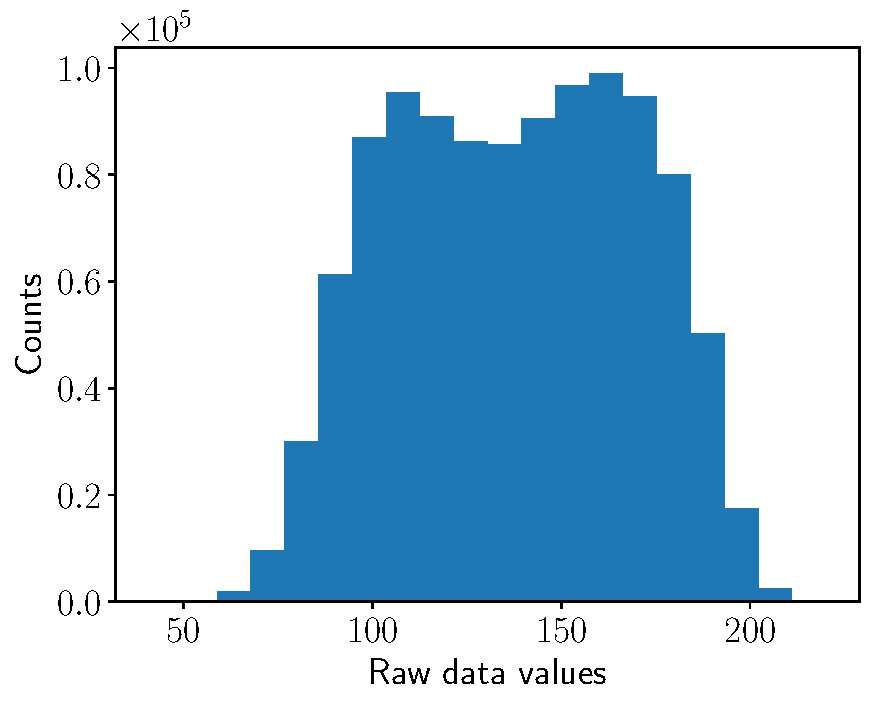
\includegraphics[width=0.85\textwidth]{raw_data_dist.pdf}
        \caption{all labels}
    \end{subfigure}
    \begin{subfigure}{0.49 \textwidth}
        \centering
        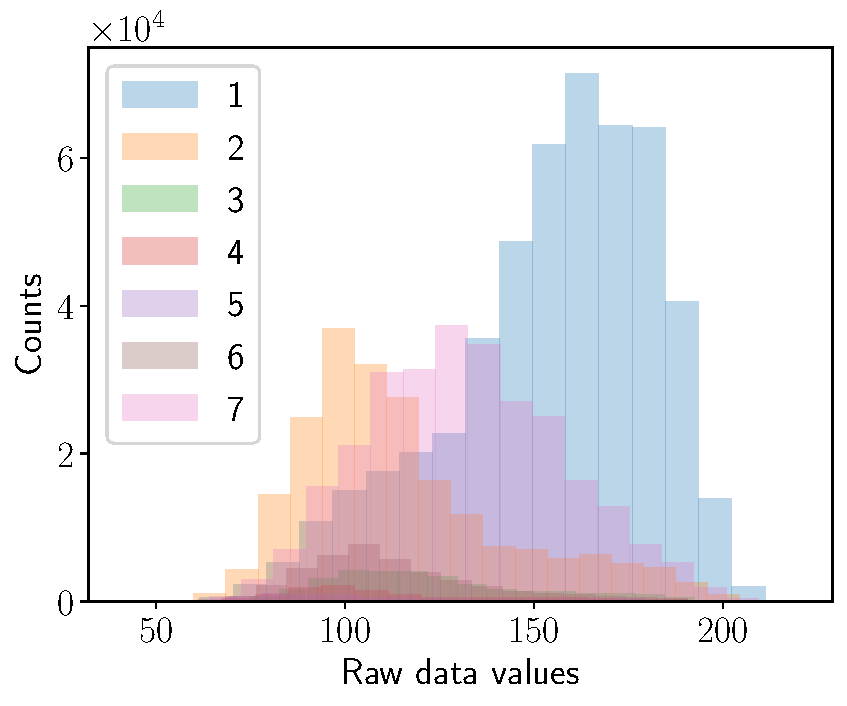
\includegraphics[width=0.85\textwidth]{raw_data_dist_per_label.pdf}
        \caption{grouped by label}
    \end{subfigure}
    \caption{The distribution of raw data for train split}
    \label{fig:dist_raw_train}
\end{figure*}

Data have a property of a high class imbalance, in particular: 46\% of all training data belongs to
cell cytoplasm, 19.4 \% to cell membrane and the remaining to other labels.
Also it worth to mention that 25.8 \% of the training split is not labeled
(i.e. label undefined has been assigned) and usually non labeled regions corresponds to
the places where several labels are adjacent and it is not clear to which class pixel should belongs to.
Therefore the hardest regions of the volume are not labeled and it can affect the performance of models
trained on this data since we use an inductive learning approach.
The distribution of the class labels for the train split is depicted on figure \ref{fig:dist_labels}.

Then we analyzed the distribution of raw data values for the train split. The histograms
are shown on figure \ref{fig:dist_raw_train}. Based on the fact that data look like it has
a normal distribution the results of statistical test of normality \cite{normalitytest} with a
null hypothesis that data is normally distributed have shown that data are not normally distributed
(all p values less than \( 10^{-182} \)) with very high confidence level.

Another important question which can be answered from data is whether means of raw data values
which corresponds to different labels are different. To check it we used several statistical tests.
First of all we compute p value for one way ANOVA \cite{lowry2014concepts} test with null hypothesis that all means are equal.
The computer p value of this test is close to 0, so not all means are equal. Then we used t-test \cite{student1908probable}
with a null hypothesis that two means are equal for every pair of data which corresponds to different labels.
The results are shown in the table \ref{tab:data_ttest} and with a high confidence level
all means are different except means for cell membrane and mitochondrion membrane. It means that in average the
raw data values of each class except this two are different and therefore a model can exploit it.

\begin{table}[ht]
    \centering
    \begin{tabular}{c|c|c|c|c|c|c|c}
        % \hline
          & 1 & 2     & 3 & 4      & 5      & 6 & 7      \\
        \hline
        1 & 0 & 0     & 0 & 0      & 0      & 0 & 0      \\
        \hline
        2 & 0 & 0     & 0 & 0.175  & 0      & 0 & 0      \\
        \hline
        3 & 0 & 0     & 0 & 0      & 0      & 0 & 0      \\
        \hline
        4 & 0 & 0.175 & 0 & 0      & 0      & 0 & 0.0003 \\
        \hline
        5 & 0 & 0     & 0 & 0      & 0      & 0 & 0.0029 \\
        \hline
        6 & 0 & 0     & 0 & 0      & 0      & 0 & 0      \\
        \hline
        7 & 0 & 0     & 0 & 0.0003 & 0.0029 & 0 & 0      \\
        % \hline
    \end{tabular}
    \caption{P-values of t-test for different labels combination}
    \label{tab:data_ttest}
\end{table}

\section{Related work}
Since the labeled dataset is unique in terms of amount of labeled data and labels
and have not been used before there are no papers which aims to solve exactly the same problem.
But a lot of approaches have been developed for similar connectomics volume images.

The paper \cite{lucchi2013learning} from where the raw data comes from solves the problem of mitochondria segmentation (binary).
Authors used non neural network based approach which use conditional random fields (CRF). They proposed
the new learning algorithm which approximate subgradients used for graphical model training using working sets and archive SOTA
results in comparison to other non neural network based methods (at least as for time of publication).
The proposed methods works on the feature vectors extracted from SLIC supervoxels \cite{achanta2012slic}
using Ray descriptors \cite{lucchi2011supervoxel} and intensity histograms.

In the last decade with a growing of popularity of neural networks a lot of CNN based
models appear in the field of connectomics volume images segmentation. Usually architectures of
segmentation networks is an adapted to 3D case version of popular 2D CNN models of they aim to work
with input subvolume or 2D CNN in a case when input is 2D image, but the later suffers from
the fact that it doesn't use all available volume information.

For example, V-Net \cite{milletari2016v}
is an adapted version of popular U-Net \cite{ronneberger2015u}, where authors swap 2D convolution with
3D convolution with kernel size \( 5 \times 5 \times 5 \) and change the number of layers for each stage from 2 to 3 as well as
downsampling strategy from pooling to strided convolutions.

In \cite{cheng2017volume} authors studied a problem of class imbalance and proposed their own loss function.
The paper considers 3D and 2D CNN models and proposed factorized to handle the computational expensiveness of 3D convolutions.
Also they pointed out the importance of augmentation such as flips and elastic deformation.

\cite{lin2021pytorch} is a python library for connectomics segmentation which implements a lot of
SOTA CNN based methods and allows users train and infer pretrained models on their data.

The shared limitation of all CNN based methods is the constraint that the output shape of the model
is equal to input shape, therefore to train a model to segment volumes the labeled volumes are required.

\section{Methodology}
Before discussing approaches which we use in our project le'ts formalize the problem. In this
research we consider only supervised methods which requires labeled data.

First of all, despite the need of multi label classification mentioned in the previos section
where for every input volume a model outputs several labels we can't come up with a
supervised solution. The reason is that even if we managed to construct and train a model for multi label
classification we still don't have any data to properly evaluate it. Therefore we end up only with multi class classification.

Secondly, the given labeled dataset contains unlabeled data (i.e. labeled with label 7) thus
there is no sense to train a model to predict class which corresponds to label 7, therefore we filter
out all examples which have this label.

Third, to use all spatial information from data the input to models will be a 3D subvolume,
but since we have only 3 labeled flat slices in the train split we cannot have a model for which
output shape equals to an input shape. The universal solution to this problem is to predict label
only for the center voxel of the input volume.

Finally the formulation of the problem is the following:
\begin{definition}
    Let \( I = [0, 1] \) be a set of normalized values
    of intensities of connectomics volume, \( Y = \{ 1, \dots, 6 \} \) -- set of labels,
    \( k \) -- subvolume size parameter, \(f_{\theta}: Q \times I^{2^k \times 2^k \times 2^k} \to Y \) -- model
    with parameter \( \theta \in \Theta \).
    Given a labeled dataset,
    \(\mathcal{D} = \{ (x_i, y_i) | x_i \in I^{2^k \times 2^k \times 2^k}, y_i \in Y \}\),
    where \( x_i \) -- subvolume of size \( 2^k \times 2^k \times 2^k \) and
    \( y_i \) -- a label of the voxel of subvolume
    \( x_i \) with index \( (2^{k-1},2^{k-1},2^{k-1}) \) (center voxel) and the loss functional
    \( \mathcal{L}: Q \times I^{2^k \times 2^k \times 2^k} \times Y \to \mathbb{R}_+ \cup \{ 0 \} \).
    The center voxel classification task is to find such as model parameter \( \theta' \in \Theta \) that:
    \begin{equation*}
        \theta' = \arg \min\limits_{\theta \in \Theta} \frac{1}{|\mathcal{D}|} \mathcal{L}(f_{\theta}(x_i), y_i)
    \end{equation*}
\end{definition}
Throughout our project we will vary model \( f \) but the formulation will remain exactly the same.

The task description \cite{proj_tasks} of this project also recommends to analyze possibilities of augmenting dataset
by generating artificial data (mask and volumes) with use of other models. Generative adversarial networks
(GANs) (e.g. CycleGAN \cite{zhu2017unpaired}) is usually used for this task and it has been proven that in such a way
augmented datasets can improve the performance of the model \cite{shumilo2023generative,sandfort2019data}.
But despite that all problems with GANs, like
unstable training, mode collapse (which is not harmful for our task, because connectomics
volume images have similar structure and properties) the issues that generated data
may have a worse quality than real, can be solved, we still can not used them.
The reason is that if we aim to generate artificial labels we need to train a discriminator to
distinguish between real and fake masks. But since we have only 3 labeled slices in the train split,
i.e. only 3 mask examples, we don't have enough data to train it.

\subsection{Probation of classical approaches}
The first type of models are inspired by the result of data analysis and in particular the result
(table \ref{tab:data_ttest}) that difference of means of almost all classes are statistically significant.
So it is worth to check whether the value of intensity of voxel itself is enough to predict a correct label.

We d o it in the following way: take intensities of all labeled voxels and train a
classical ML models such as:
\begin{itemize}
    \itemsep0em
    \item Decision tree \cite{breiman2017classification}
    \item Random forest \cite{breiman2001random}
    \item Ada boosting on trees \cite{hastie2009multi}
    \item Gradient boosting on trees \cite{friedman2001greedy}
\end{itemize}
Since it is clear that only intensities probably will not be enough to correctly predict
labels we use the same list of models but extend inputs by adding a hand crafted features by
applying well known convolutional kernels to the train slices, in particular:
\begin{itemize}
    \itemsep0em
    \item Sobel's \(x \) and \(y\) derivatives
    \item Prewitt's \(x \) and \(y\) derivatives
    \item Laplace
    \item Gradient magnitudes from sobel and prewitt gradients
\end{itemize}
But as it will be shown in the subsection \ref{sec:voxelwise_expr} even these features are
not enough to perform segmentation with appropriate quality therefore we need more complex models
and extension of inputs to subvolumes.

\subsection{Convolutional neural networks}

\begin{figure}[t]
    \centering
    \begin{subfigure}[t]{0.2 \textwidth}
        \centering
        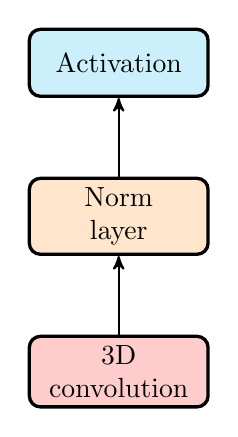
\begin{tikzpicture}[
                module/.style={draw, very thick, rounded corners, minimum
                        width=15ex},
                conv/.style={module, minimum height = 0.85cm, fill=red!20},
                norm/.style={module, minimum height = 0.85cm, fill=orange!20},
                act/.style={module, minimum height = 0.85cm, fill=cyan!20},
                arrow/.style={-stealth', thick, rounded corners},
            ]

            \node[conv, align=center] (conv_layer) {3D \\ convolution};
            \node[above=of conv_layer, norm, align=center] (norm_layer) {Norm\\layer};
            \node[above=of norm_layer, act, align=center] (activation) {Activation};

            % \node[fit={(mha)(addnorm2)(mharesidual)(ln1residualleft)}
            %     draw, ultra thick, rounded corners,
            % ] (encoder) {};

            \draw[arrow] (conv_layer) -- (norm_layer);
            \draw[arrow] (norm_layer) -- (activation);
        \end{tikzpicture}
        \caption{Convolutional block}
        \label{fig:conv_block}
    \end{subfigure}
    \hfill
    \begin{subfigure}[t]{0.28 \textwidth}
        \centering
        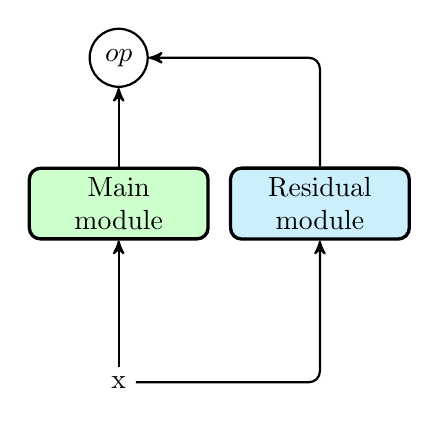
\begin{tikzpicture}[
                module/.style={draw, very thick, rounded corners, minimum
                        width=15ex},
                main/.style={module, yshift = 0.6cm, minimum height = 0.85cm, fill=green!20},
                res/.style={module, xshift = -5ex, minimum height = 0.85cm, fill=cyan!20},
                arrow/.style={-stealth', thick, rounded corners},
            ]

            \node[align=center] (input) {x};
            \node[above=of input, main, align=center] (main_module) {Main \\ module};
            \node[right=of main_module, res, align=center] (res_module) {Residual \\ module};
            \node[above=of main_module, draw, thick, circle] (res_op){$op$};

            \draw[arrow] (input) -- (main_module);
            \draw[arrow] (input) -| (res_module);
            \draw[arrow] (main_module) -- (res_op);
            \draw[arrow] (res_module) |- (res_op);
        \end{tikzpicture}
        \caption{Residual block}
        \label{fig:res_block}
    \end{subfigure}
    \caption{CNN building blocks}
    \label{fig:blocks}
\end{figure}

The next type of models is 3D convolutional neural networks (CNN) which have shown their efficiency
on the similar connectomics segmentation tasks. We have implemented a variety of architectures for our
research. In total we end up with 6 different types of architectures.
The basic building blocks of almost all models is depicted on the figure \ref{fig:blocks}.
In order to describe it let's introduce the notation:
\begin{itemize}
    \itemsep0em
    \item Conv3D[\( kernel, stride, padding, dilation, feat, norm, \) \( act\)] -- convolution block as on the figure \ref{fig:conv_block}
          where 3D convolution layer has corresponding kernel size, padding, size and dilation, with  equals
          number of output features is \( feat \), normalization layer is
          as it described by \( norm \) and activation is \( act \).
    \item Conv3D[\( feat \)] -- convolution block of specific type which refers to
          Conv3D[\( 3, 1, 1, 0, feat, batch, ReLU \)]
    \item Conv3DGELU[\( feat \)] -- convolution block of specific type which refers to
          Conv3D[\( 3, 1, 1, 0, feat, batch, GELU \)]
    \item Conv3DGELUPad[\( feat \)] -- convolution block of specific type which refers to
          Conv3D[\( 3, 1, 1, 1, feat, batch, GELU \)]
    \item Conv3DGELUPad[\( feat \)] -- convolution block of specific type which refers to
          Conv3D[\( 3, 1, 1, 1, feat, batch, GELU \)]
    \item Conv3DLNPad[\( feat \)] -- convolution block of specific type which refers to
          Conv3D[\( 3, 1, 1, 1, feat, layer, GELU \)]
    \item Res[\( MainModule, ResModule, Op \)] -- residual module as on the figure \ref{fig:res_block}.
    \item Res[\( MainModule \)] -- default residual module which refers to Res with indentity \( ResModule \) and
          summation as an operation
    \item Res2Conv[\( feat \)] -- residual module with 2 convolutional blocks with GELU activation:
          Res[\( Conv3DGELUPad[feat] - Conv3DGELUPad[feat] \)]
    \item Res2ConvLN[\( feat \)] -- residual module with 2 convolutional blocks with GELU activation and layer norm:
          Res[\( Conv3DLNPad[feat] - Conv3DLNPad[feat] \)]
    \item Concat[\( MainModule, ResModule\)] -- residual module where operation \( Op \) is a concatenation along the channel axis
    \item AvgPool -- average 3D pooling with kernel size \( 2 \) and stride \( 2 \)
    \item MaxPool -- maximum 3D pooling with kernel size \( 2 \) and stride \( 2 \)
\end{itemize}

All our architectures differs only in backbones (features extractors) whereas the head always
has the same architecture: it is a linear layer represented as an usual 3D convolution with kernel size
equals to the shape of features of the output of the backbone. We have the following custom backbones
(input shape refers to the size along the one dimension):
\begin{table}[ht]
    \begin{tabular}{p{1.2cm}p{1cm}p{5.3cm}}
        Name      & Input shape & Architecture                                                                                                                                                         \\
        \toprule
        3layer    & 8           & Conv3D[16] - Conv3D[32] - Conv3D[64] - AvgPool                                                                                                                       \\
        \hline
        4conv     & 32          & Conv3DGELU[16] - MaxPool - Conv3DGELU[32] - MaxPool - Conv3DGELU[64] -- Conv3DGELU[128] - AvgPool                                                                    \\
        \hline
        4conv\_ln & 32          & Conv3DLN[16] - MaxPool - Conv3DLN[32] - MaxPool - Conv3DLN[64] -- Conv3DLN[128] - AvgPool                                                                            \\
        \hline
        4res      & 16, 32      & Conv3DGELUPad[16] - MaxPool - Conv3DGELUPad[32] - Res2Conv[32] - MaxPool - Conv3DGELUPad[64] - Res2Conv[64] - MaxPool - Conv3DGELUPad[128] - Res2Conv[128] - AvgPool \\
        \hline
        4res\_ln  & 16, 32      & Conv3DLNPad[16] - MaxPool - Conv3DLNPad[32] - Res2ConvLN[32] - MaxPool - Conv3DLNPad[64] - Res2ConvLN[64] - MaxPool - Conv3DLNPad[128] - Res2ConvLN[128] - AvgPool   \\
        \hline
        dil16     & 16          & Conv3D[16] - Concat[Conv3D[3, 1, 0, 3, 32, batch, RELU] -- Conv3D[5, 1, 0, 3, 32, batch, RELU]] --  AvgPool                                                          \\
        \hline
        dil       & 32, 64      & Conv3D[16] - MaxPool - Concat[Conv3D[3, 1, 0, 3, 32, batch, RELU] -- Conv3D[5, 1, 0, 3, 32, batch, RELU]] --  AvgPool                                                \\
        \bottomrule
    \end{tabular}
    \caption{Architectures of handcrafted backbones}
    \label{tab:arch}
\end{table}

In short words, \textit{3layer} and \textit{4conv} models is just a simple CNNs where
after every convolutional block we have a downsampling pooling layer, prefix \textit{ln} means using layer normalization
instead of class batch. \textit{4res} is a 4 stage ResNet where every ResNet block consists of
two sequential convolutional blocks, we use another convolutional block to change the dimensionality
of features after every downsampling with pooling layers. And finally \textit{dil} models contain
a pyramid of features produced by dilated convolutions (with dilation \( 3 \))
for different kernel sizes: two \( 3 \times 3 \) and one \( 5 \times 5 \),- inspired by \cite{chen2017deeplab} and aims to have bigger
reception field and handle the problem that adjacent voxels of connectomics usually similar to each other.
The \textit{dil16} model differs from other only in missing max pooling after first convolutional block.

In addition to handcrafted backbones we adapt state of the art CNN model ConvNext \cite{liu2022convnet} to 3D
case by changing 2D convolution with 3D counterparts. For an input shape \( 32 \times 32 \times 32 \) we
reuse exactly the same model architecture as ConvNext-tiny, whereas for \( 16 \times 16 \times 16 \) input's shape we
changed patch size from \( 4 \) to \(2 \).

As a loss function we use two options: classical cross entropy loss and adapted FocalLoss from
RetinaNet \cite{lin2017focal} which designated to handle a high class imbalance.

\subsection{Tiled prediction}
Another point which is worth to discuss is ability to make a tiled prediction,
i.e. without changing a model get as an input extended subvolume and output
predictions not only for the center voxel but for center region in accordance to extension of the input,
e.g. if model standard input has a shape \( 32 \times 32 \times 32 \) pass subvolume with a shape
\( 33 \times 33 \times 33 \) and get \( 2 \times 2 \times 2 \) prediction for a center region.
We investigated this problem and end up with a conclusion that usually it is not possible:
the reason is downsampling layers which have strides greater than 1 (usually 2) and are present in
every our CNN architecture. If we want to predict a label for adjacent center voxel we have
to have a stride 1, but then further layers will have a wrong input features. We can solve it for convolutional
layers with use of dilation equal to the stride of the previous downsampling layer, but only until the next layer
with stride greater than 1 whereas we always have several downsampling layers in out networks.

The easiest way to prove it is to think in terms of a shape of the outputs of a CNN backbone and input features:
we just add \( m \in \mathbb{N} \) pixel to an input along one or several dimension, but every downsampling layer divide a
shape of features by \( n \in \mathbb{N} \) times (e.g. layers with stride 2 half every feature spatial axis shape)
therefore the final features from the backbone won't be equal to the number of features for standard input plus extension (\(m\)).

\subsection{Pretraining}
Initially pretraining approaches such as masked token prediction \cite{devlin2018bert}
or next token prediction \cite{radford2019language}
have shown their efficiency for NLP tasks. The main idea is to use only
unlabeled data and train model to predict some masked part of it which allows model
to better understand the structure of data (language) and only then finetune model on labeled
dataset to some specific task.
In the last years it has been proved \cite{woo2023convnext} that CNN models also can benefit from
pretraining in the similar way, i.e. by masking part of the image with the aim
of its reconstruction via autoencoder.

Inspired by this ideas we propose 2 types of pretraining techniques for out task.
It is possible because every CNN can be split into 2 parts: backbone which extract
features and head which depends on the task. So, during the pretraining we will train
the backbone of the model and then during finetuning stage change the head to classification.
Therefore all our pretraining methods differs only in heads.

The first pretraining method is a center voxel regression. We mask the center voxel
(optionally with padding, e.g. if padding 1 then we mask \( 3 \times 3 \) center region)
and train our model to predict the intensities in the masked region. This method is based
on the findings from section \ref{sec:data_analysis} that means of intensity for almost all classes are different therefore intensity itself
can help to predict a correct label.

The second approach is a training of the variational autoencoder (VAE) \cite{kingma2013auto} where we
optionally mask the center voxel (optionally with padding, i.e. some center region) and reconstruct the whole input (including the masked
center region) using VAE framework. This approach is adapted from \cite{woo2023convnext} but we
optionally mask interesting for us center voxel/region and usually use different network architecture.

\subsection{Postprocessing}
Since models predict a label for a particular voxel independently
(adjacent voxels only shares part of an input) it is possible that the final predicted
mask for the whole volume will be non consistent, i.e. similar, close to each voxel will have
a different labels and the whole output will look noisy. Some 2D CNN segmentation models, like DeepLab \cite{chen2017deeplab},
solve this issue by using CRF model on the predictions of a model. But whereas the usual approach
to smooth predictions is a local CRF (which work on a voxel and its neighborhood), we use a fully connected CRF,
i.e. CRF where every voxel of the predicted volume is connected. This
will allows us to guarantee not only a local consistency, but capture a global structure as well.

But since solving the discrete optimization problem for fully connected graph for meaningful
size of volume can become computationally intractable we constrained the CRF model to have
a specific type which can be solved efficiently, i.e. CRF with gaussian edge potentials \cite{krahenbuhl2011efficient}.

The energy function for this CRF is the following:
\begin{equation*}
    E(\mathbf{x}) =\sum\limits_{i \in V} \theta_i (\mathbf{x_i}) +
    \sum\limits_{ij \in E} \theta_{ij} (\mathbf{x_i}, \mathbf{x_j})
\end{equation*}
where \( G = (V, E) \) -- complete graph where every voxel \( v \in V \) is a node,
\(\mathbf{x}_i \in \{0, 1\}^{|Y|} \) -- one hot encoding of labeling of the voxel \( i \) (\(Y\) -- set of labels),
\( \theta_i = -\ln{p_i} \) -- unary term depended on the predicted probabilities \( p_i \) of labels,
\(\mathbf{x} = (\mathbf{x_i} | i \in V) \) -- the whole labeling.
And the crucial element of the model which allows us to efficiently infer it is the pairwise term:
\begin{equation}  \label{eq:crf_pairwise_term}
    \begin{aligned}
        \theta_{ij} (\mathbf{x_i}, \mathbf{x_j}) = \mu_1(\mathbf{x_i}, \mathbf{x_j})
        \exp \left( -\frac{\| l_i - l_j \|^2}{2 \theta_{\alpha}^2}
        -\frac{\| I_i - I_j \|^2}{2 \theta_{\beta}^2} \right) + \\
        \mu_2 (\mathbf{x_i}, \mathbf{x_j}) \exp \left( -\frac{\| l_i - l_j \|^2}{2 \theta_{\gamma}^2} \right)
    \end{aligned}
\end{equation}
where \( \mu_k(\mathbf{x_i}, \mathbf{x_j}): \{0, 1\}^{|Y|} \times \{0, 1\}^{|Y|} \to \mathbb{R}, k \in \{ 1, 2 \} \)
-- labels incompatibility term, \( l_i \) -- location of the voxel \( i \) in the volume,
\( I_i \in [0, 1] \) -- normalized intensity of voxel \( i \),
\( \theta_{\alpha}, \theta_{\beta}, \theta_{\gamma} \in \mathbb{R}_+ \) -- parameters of the
importance of corresponding difference in intensity and location.

This method of postprocessing is to be applied to the whole slices which we have in the dataset during training and
evaluation and to subvolumes when model generate predictions for the whole raw data volume because of memory limits.

\section{Experiments}
In order to compare different model architecture and study impact of input volume size and pretraining we
have conducted a lot of experiments. All experiments that involves CNNs have been run on NVIDIA A100 with 40GB of GPU memory
and used Adam optimizer with parameters \( \beta_1=0.9, \beta_2=0.999 \), the weight decay was \( 5 \dot 10^{-4} \)
and the learning rate was set to \( 10^{-3} \). We have measured a lot classification metrics for every
particular class as well as overall, such as precision, recall, F1, AP (average precision) and cohen kappa,
but in this section we will show only overall metrics on the test split: averaged F1, AP and cohen kappa (\(\varkappa\)).

For this research project we have written fully configurable via yaml files code which is available under the following
link\footnote{\url{https://github.com/ShkalikovOleh/connectomics_segmentation}}.

\subsection{Classical voxelwise models} \label{sec:voxelwise_expr}
First of all we have evaluated voxelwise classical ML models in order to check whether they are powerful enough to
correctly predict labels. In order to do this we train using Scikit-Learn \cite{scikit-learn} all described above
voxelwise models with default hyperparamets on 1 train slice (in the XZ plane)
and evaluate them on 1 test slice (in the YZ plane). The results of evaluation are given in the table
\ref{tab:voxelwise_metrics}.

\begin{table}[ht]
    \centering
    \begin{tabular}{|c|c|c|c|c|c| }
        \hline
        \textbf{Model}                 & \textbf{Features} & \textbf{F1}    & \textbf{AP}    & \( \mathbf{\varkappa} \) \\
        \hline
        \multirow{2}{*}{Decision tree} & 1                 & 0.278          & 0.345          & 0.656                    \\
                                       & 8                 & 0.317          & 0.261          & 0.584                    \\
        \hline
        \multirow{2}{*}{Random forest}
                                       & 1                 & 0.278          & 0.345          & 0.655                    \\
                                       & 8                 & \textbf{0.319} & 0.315          & 0.618                    \\
        \hline
        \multirow{2}{*}{AdaBoost}
                                       & 1                 & 0.277          & 0.219          & 0.654                    \\
                                       & 8                 & 0.281          & 0.212          & \textbf{0.671}           \\
        \hline
        \multirow{2}{*}{GradientBoost}
                                       & 1                 & 0.278          & 0.346          & 0.656                    \\
                                       & 8                 & 0.282          & \textbf{0.355} & 0.676                    \\
        \hline
    \end{tabular}
    \caption{Metrics for voxelwise models}
    \label{tab:voxelwise_metrics}
\end{table}

From values of F1 we can conclude that models trained on handcrafted features outperform their counterparts
which used only the intensity values, but as it follows from AP and cohen kappa these models (in particular random forest and decision tree)
are less confident in their predictions. The analysis of per class metrics shows us the crucial problem of all these models: they all have a good predictions
only for 2 top class whereas all other sometimes even not present in the output of the model. Also it is worth to mention that
these models are overfited to the train dataset, because metric values are usually 2 times higher for the train split.

The results shows us that we really need more complex models and extended to subvolume inputs, because segmentation
scores are relatively low.

\subsection{Segmentation models evaluation}

In total by varying architectures, losses and hyperparameters we have trained and evaluated 35 CNN models.
The metrics for top 5 model according to the averaged F1 are denoted in the table \ref{tab:cnn_raw_metrics}.
All logs of experiments are available under the following link\footnote{\url{https://wandb.ai/shkalikov-oleh/connectomics_segmentation}}.

\begin{table}[ht]
    \centering
    \begin{tabular}{|p{1.2cm}| >{\centering\arraybackslash}p{1cm}|c|c|c|c|c|}
        \hline
        \textbf{Model} & \textbf{Input shape} & \textbf{Loss} & \textbf{F1}    & \textbf{AP}    & \( \mathbf{\varkappa} \) \\
        \hline
        4res           & 32                   & CE            & \textbf{0.913} & \textbf{0.962} & \textbf{0.939}           \\
        \hline
        4conv          & 32                   & CE            & 0.906          & 0.952          & 0.938                    \\
        \hline
        4res\_ln       & 32                   & CE            & 0.905          & 0.959          & 0.937                    \\
        \hline
        dil            & 32                   & CE            & 0.885          & 0.95           & 0.923                    \\
        \hline
        4res           & 16                   & CE            & 0.883          & 0.933          & 0.926                    \\
        \hline
    \end{tabular}
    \caption{Metrics for top 5 CNN models}
    \label{tab:cnn_raw_metrics}
\end{table}

The best model according to the conducted experiments is a ResNet \textit{4res} as it is described in the table \ref{tab:arch} with
an input shape \( 32 \times 32 \times 32 \) trained with cross entropy loss. Moreover, the same model we have on the 3 and 5 places but
with different input shapes and normalization layers.

The analogon of SOTA 2D classification model \textit{ConvNext} perform by far worse than proposed handcrafted backbones, in particular the
best model of this type which was trained with CE loss on the input volumes with a shape \( 32 \times 32 \times 32 \) have only
0.741 averaged F1 score. The main reason for this is a poor performance on the minor class. The possible explanation is the fact, that
bigger model requires more diverse and bigger dataset in order to train all their weights. Thus we can conclude that smaller models
is more performant that bigger ones for out task.

Surprisingly all models which was trained with FocalLoss (with parameters \( \gamma = 2 \) and \( \gamma=4 \) have a worse metric values than exactly the same models trained with
cross entropy. In the situation when we have such an class imbalance it was expected to get an opposite results. One of the possible
explanation is a incorrect implementation of the loss or the fact that we haven't test all values of loss hyperparameters.

Also it worth to mention that since a lot of the most interesting, the hardest to classify voxels have not been labeled in the given slices,
we cannot fully rely on the computed metrics, because even if our model misclassify all complicated regions but return the correct labels for
labeled in the dataset voxels we still will have a high values of metrics.


\subsection{Efficiency of pretraining}

Since the pretraining make sense mostly for big models we evaluate the efficiency of pretraining techniques
on \textit{ConvNext} architecture. The results are given in the table \ref{tab:pretraining_comparison}.

\begin{table}[ht]
    \centering
    \begin{tabular}{|c| >{\centering\arraybackslash}p{1cm}|c|c|c| }
        \hline
        \textbf{Model}            & \textbf{Pretr. type} & \textbf{Input shape} & \textbf{Loss} & \textbf{F1}    \\
        \hline
        \multirow{3}{*}{ConvNext} & CR1                  & \multirow{3}{*}{32}  & CE            & \textbf{0.741} \\
                                  & CR0                  &                      & CE            & 0.682          \\
                                  & -                    &                      & CE            & 0.701          \\
        \hline
        \multirow{3}{*}{ConvNext} & CR0                  & \multirow{3}{*}{32 } & Focal2        & \textbf{0.687} \\
                                  & -                    &                      & Focal2        & 0.5312         \\
                                  & -                    &                      & Focal4        & 0.492          \\
        \hline
        \multirow{2}{*}{ConvNext} & CR1                  & \multirow{2}{*}{16 } & CE            & 0.603          \\
                                  & -                    &                      & CE            & \textbf{0.728} \\
        \hline
    \end{tabular}
    \caption{Comparison of ConvNext models with and without pretraining. CR\(N\) means center voxel regression
        with padding equals to \(N\) and
        Focal\(A\) means the Focal Loss with \( \gamma = A \).}
    \label{tab:pretraining_comparison}
\end{table}

As we can see for both biggest models the center regression pretraining have managed to improve the performance of the
finetuned model. Another interesting note is that masking with non zero padding works better than just masking the center voxel and random
voxels (in this case with dropout probability \( 0.3 \)) which can be explained by the fact that adjacent pixels in the
connectomics usually are similar to each other and therefor during pretraining we fit models just to copy the value of
non masked adjacent to the center voxel.



\begin{figure*}[t]
    \begin{subfigure}{0.49 \textwidth}
        \centering
        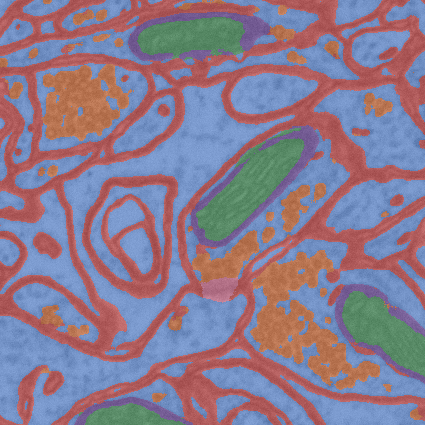
\includegraphics[width=0.6\textwidth]{raw_pred.png}
        \caption{raw predictions}
    \end{subfigure}
    \begin{subfigure}{0.49 \textwidth}
        \centering
        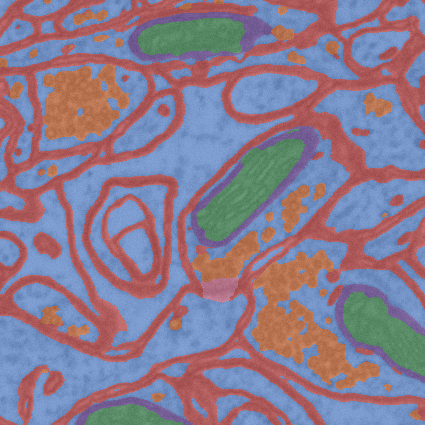
\includegraphics[width=0.6\textwidth]{crf_pred.png}
        \caption{CRF postprpocesed}
    \end{subfigure}
    \caption{Comparison of raw and postprpocesed prediction of the best CNN model \textit{4res} trained with CE loss
        with an input shape \( 32 \times 32 \times 32 \) for the test slice in the XY plane}
    \label{fig:crf_comparison}
\end{figure*}

\subsection{Postprocessing quality}

In order to evaluate the quality of postprocessing we the predictions of the CNN models and pass them apply described above
CRF model to them with the following parameters: \( \theta_{\alpha}=\theta_{\beta}=\theta_{\gamma} = 1 \) and incompatibility
term for the bilateral term (first term of \eqref{eq:crf_pairwise_term}) was equal to
\begin{align*}
    \Upsilon = \begin{pmatrix}
                   0   & 1.0 & 100 & 1.0 & 1.0 & 100 \\
                   1.0 & 0   & 100 & 10  & 0.5 & 100 \\
                   100 & 100 & 0   & 5.0 & 100 & 100 \\
                   1.0 & 10  & 5.0 & 0   & 100 & 100 \\
                   1.0 & 0.5 & 100 & 100 & 0   & 100 \\
                   100 & 100 & 100 & 100 & 100 & 0   \\
               \end{pmatrix} \\
    \mu_1(\mathbf{x_i}, \mathbf{x_j}) = \Upsilon_{\arg \max \mathbf{x_i}, \arg \max \mathbf{x_j}}
\end{align*}
and for the second term of \eqref{eq:crf_pairwise_term} we use simple Potts model where
\( \mu_2(\mathbf{x_i}, \mathbf{x_j}) = 1 \) if and only if the labels \( \mathbf{x_i}, \mathbf{x_j} \) are different.

All this parameters have been found imperially by comparing outputs of CRF models. The metrics for the postprpocesed predictions of top 5 models can be found in the table \ref{tab:cnn_crf_metrics}.

\begin{table}[ht]
    \centering
    \begin{tabular}{|p{1.2cm}| >{\centering\arraybackslash}p{1cm}|c|c|c|c|}
        \hline
        \textbf{Model} & \textbf{Input shape} & \textbf{Loss} & \textbf{F1}    & \( \mathbf{\varkappa} \) \\
        \hline
        4res           & 32                   & CE            & 0.901          & \textbf{0.937}           \\
        \hline
        4conv          & 32                   & CE            & \textbf{0.902} & 0.935                    \\
        \hline
        4res\_ln       & 32                   & CE            & 0.897          & 0.93                     \\
        \hline
        dil            & 32                   & CE            & 0.828          & 0.868                    \\
        \hline
        4res           & 16                   & CE            & 0.878          & 0.922                    \\
        \hline
    \end{tabular}
    \caption{Metrics for postprpocesed outputs of top 5 CNN models}
    \label{tab:cnn_crf_metrics}
\end{table}

Based only on the metrics the postprpocesed results are worse, but actually if we look at the result it is even better,
e.g the figure \ref{fig:crf_comparison}. The postprpocesed precisions more structurally correct, i.e. CRF has closed mitochondria
membranes and after postprocessing all mitochondria surrounded by membranes. Also CRF has replaced wrongly predicted
to vesicles labels in the right bottom mitochondrion to the proper mitochondrion labels.

\section{Directions of further research}

The obvious further steps which related to the proposed CNN approach are developing other
network architecture, hyperparameter search, using other loss functions suitable for
datasets with a high class imbalance, learning parameters of CRF model.

But one of the main drawback of the discussed method is that we don't use any constraints induced by
biological properties of labels to make predictions, e.g. mitochondrion always surrounded by
mitochondrion membranes.

\subsection{Context-free formal grammars}
One of the promising approach to use this information is 2D/3D context free grammars. In the analysis of texts
formal grammars are being used to detect whether the given text has a suitable structure defined by grammar rules.
The context free grammars have a specific form of rules which in Chomsky normal form could be represented as a
renaming a non-literal symbol to a literal and concatenation of two non-literals.

Cocke–Younger–Kasami (CYK) algorithm \cite{sakai1961syntax} for the given grammar an input text can predict whether the text
can be generated by the grammar. It do it by trying to construct on every step \( m \) all substrings in accordance to the rules from all
substrings constructed on the previous step and symbols of the input text. The input text could be generated be grammar
if and only if algorithm managed to construct substring which equals to the input text.

\cite{schlesinger2013ten} have shown that usual context free grammar can be extended to N dimension
case as well as CYK algorithm. The idea is to come with a grammar which match the structural properties of
connectomics. Then we can use this grammar in two possible ways: to evaluate whether
a prediction for the whole volume is structurally correct and to correct wrong predictions.
The latter can be implemented in the following way: instead of using binary grammar (where rules outputs binary value) we can use stochastic context-free grammar where literals (predicted probabilities)
and outcomes of rules are represented as a real number in a range \( [0, 1] \). If the outcome for the whole input volume will below the threshold
value, which means that the structure of the predictions is not correct, we can use the property of CYK algorithm and backtrace
to a literal which have higher impact on the result by going through the derivation path with the lowest probabilities and then change it.
This approach could be used (semi-)unsupervised training or even for generating an artificial training data in the teacher-student setup where the teacher model
labels an arbitrary input volume and then it is used for training a student model.

The main problem with implementing this idea is the fact that it hard to list all possible rules that describes
biological structural properties with voxels as literals because they very features become intractable with the growing of
the volume shape.

\section{Conclusions}

The given labeled dataset has several limitations such as limited size, high class imbalance, existence of non labeled regions
in the most complicated parts of dataset's slices what doesn't allow model to train on them and doesn't allow us to evaluate models on them.
In order to overcome some of these issues we have proposed 6 types of CNN models, pretraining techniques such as center voxel regression and
using of VAE, different variation of loss such as classical cross entropy and Focal loss, postprocessing step with use
of CRF model.

It has been shown that classical voxelwise models perform bad on the given data even when we added
additional features generated by applying several filters to the input of the model therefore using subvolumes as
an input and more complex models like CNN, which can learn to automatically extract feature from the given volume,
are justified.

We have shown that smaller networks performs better for our task and archived
the F1 score of 0.913 with ResNet model \textit{4res}. Then we managed to improve the quality in terms
of the real biological structure of the predicted labels by using
fully connected CRF on a postprocessing stage.

We argue that the further researches can benefit from using structural properties of connectomics on a postprocessing and even
a training step.

\bibliography{../references.bib}
\bibliographystyle{ieeetr}

% \onecolumn
% \section*{Appendix} \label{sec:appendix}

\end{document}